\documentclass[main.tex]{subfiles}
\begin{document}
	
	\chapter{Manipulation}
		\chapterauthor{Marc Stelter, Jan Neuman \& Fabian Weihe}
	
	\subsection{General}
	We created four Actionservers for Manipulation.\\
	The "move\_gripper\_action\_server" moves the gripper to the given position.\\
	The "perceive\_action\_server" moves the robot into perceiving position.\\
	The "grasps\_object\_server" receives the size of an object and grasps it.\\
	The "place\_server" places the attached object at the given pose.\\
	Further we've created an Launchfile, which launch the Actionservers, rviz and giskard.
	
	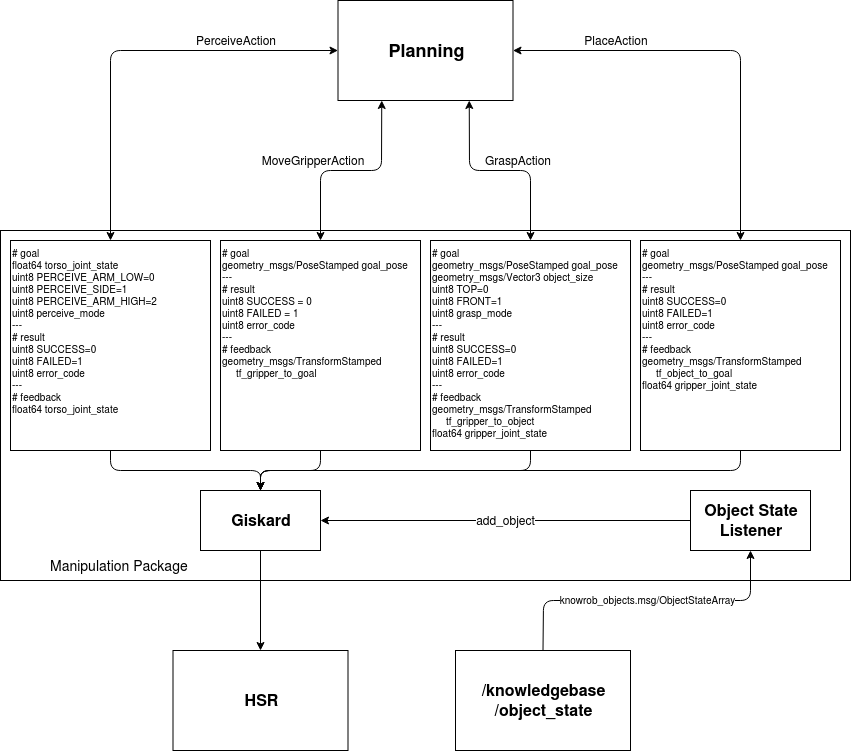
\includegraphics[scale=0.5]{subdocuments/Manipulation.png}
	
	\subsection{Move Gripper}
	The received pose is simply forwarded as a cartesian goal to giskard, which in turn will take care of the collision avoidance and movement. Giskards error\_code gets returned to the client.
	\vspace{1cm}
	
	\subsection{Perceive Position}
	The Perceive Action Server gets a float torso\_joint\_state and an int perceive\_mode from the client. The torso\_joint\_state tells the server how high the camera should be moved. The perceive\_mode describes the pose. Then the server moves all joints into a predefined pose that is chosen in perceive\_mode and the arm\_lift\_joint to the given height. When the action is finished either SUCCESS or FAILED are returned to the client.

	\vspace{1cm}
	
	\subsection{Grasps Object}
	The server receives a PoseStamped ("goal\_pose") and a Vector3("object\_size"). In the first step the script open the gripper to the maximum. After that the arm is moved to the object. If the arm moved in the given position the script closes the gripper. At the end we add the grasped object in Giskard and attach it to the robot. Finally we transform to a position, where we can comfortably move with an object in the gripper.\\
	Finally we return if the action has failed or succeeded.
	
	
	\vspace{1cm}
	
	\subsection{Place Object}
	The object to be placed needs to be attached to the gripper in giskard. Giskard is then used to move the object to its goal. In order to release the gripper the hsr python interface is used directly.
	\vspace{1cm}
	
	\subsection{Launch}
	We created a package named "launch". The package contains a Launchfile to launch the Actionservers with their dependencies. The File includes five arguments.\\
	The first one is a boolean called "sim". On false giskard is launched to work on the real robot. Otherwise on true giskard is launched to work in a simulation. Additional to that the iai\_hsr\_sim is launched for the simulation.\\
	The other four arguments are booleans, too. Which defines whether an actionserver should start. 
\end{document}
